\subsection{Featureauswahl}
\label{sec:feature_selection}
Insgesamt wurden 28 Varianten an Features untersucht und davon 3 Features verstärkt aus denen 20 Varianten entstanden sind. Die Features, die von Song et al. genutzt wurden
(siehe Tabelle \ref{tab:songFeatures}) eignen sich ohne Änderungen nicht, da sie mindestens eine Anforderung nicht erfüllen.
\newline
\newline
Das \textit{Mean absolute value} Feature ermöglicht die einzelnen Handgesten zu unterscheiden, wenn das Feature in verschiedene Zeitfenster aufgeteilt wird. Zusätzlich kann die Helligkeit normalisiert werden.
Um die Featuremenge zu verringern, können Spalten und Zeilen zusammengefasst werden. Allerdings generalisierte der Ansatz nicht gut, da die Varianz sehr groß bei Handgesten mit verschwieder Geschwindigkeit.
\newline
\newline
\textit{Average amplitude change} eignet sich gut um horizontale und vertikale Bewegungen zu unterscheiden. Allerdings ist es nicht möglich symethrische Bewegungen zu unterscheiden. Nicht untersucht wurden
Änderungen, die beim \textit{Mean absolute value} durchgeführt wurden.
\newline
\newline
Feature 2, 5 und 7 bis 9 wurden nicht weiter untersucht, weil sie zu komplexe Berechnungen bedürfen für ein kleines eingebette System ohne Modul zur Gleitkommazahlberechnung.

\subsubsection{Motion History}
Die Motion History zeigt eine Bewegungshistorie, indem eine kürzlich stattgefundene Bewegung heller ist als länger zurückliegende. Es ist invariant gegenüber Lichtverhältnisse, hat jedoch 2 große Schwachpunkte.
Einerseits kann es überlappende Bewegungen nicht richtig anzeigen, da eine kürzlich detektierte Bewegungung den Wert auf den Maximalwert $\tau$ setzt. Dies stellt in diesem Anwendungsfall kein
Problem dar, da die definierten Handgesten keine Überlappung erzeugen.
\newline
\newline
Andereseits ist das Feature bei konstantem $\tau$ und $\delta$ nicht invariant gegenüber der Geschwindigkeit. Als Lösung wurde $\delta$ abhängig von der Gestenlänge gemacht,
d. h. $\delta = \frac{\tau}{\#Bilder}$. Mit dieser Konfiguration ist die Bewegung nicht unvollständig, wenn sie langsam ausgeführt wird. Allerdings geht dieser Ansatz von einer konstanten
Ausführungsgeschwindigkeit der Handgeste aus.
\newline
\newline
Eine Bewegung in einem Pixel $q$ wird durch die Funktion \ref{formular:motion_history_phi} signalisiert, d. h. die Bewegung in $q$ findet statt, wenn eine Veränderung oberhalb des Durchschnitts detektiert wird.
\begin{align}
    \phi(q,t) = \begin{cases}
                    1 & if \Delta_{q,t} \geq \frac{1}{N} \sum_{n=1}^N \Delta_{q,n} \\
                    0 & otherwise
    \end{cases}
    \hspace{0.5cm}where\ \Delta_{q,t} = |q_t - q_{t-1}|
    \label{formular:motion_history_phi}
\end{align}

\subsubsection{Helligkeitsverteilung}
Ein Pixel $q$ ist am hellsten unter allen Pixeln in einem Bild $Q$, wenn $q$ den höchsten Wert hat. Analog ist der dunkelste Pixel, der mit dem geringsten Wert. Folglich kann der hellste Pixel als
$q' = \arg(\max Q)$, bzw. der dunkelste Pixel als $q' = \arg(\min Q)$ definiert werden.
\newline
\newline
Weiterhin wird die Bildsequenz in eine bestimmte Anzahl von gleich großen Zeitfenstern aufgeteilt. In jedem Zeitfenster wird der hellste bzw. dunkelste Pixel ermittelt. Aus der daraus resultierenden
Featuremenge kann jede definierte Handgeste inferiert werden. Sie ist invariant zu Lichtverhältnissen und Geschwindigkeiten. Per Definition gibt sie Auskunft über die Entwicklung über Zeit und die Position.
\newline
\newline
Es gibt mehrere Möglichkeiten die einzelnen Pixel in einem Zeitfenster zusammenzufassen.
\begin{itemize}
    \item Wähle das Minimum bzw. Maximum.
    \item Projeziere die Pixel auf ein kartesisches Koordinatensystem und fasse die Punkte über eine Abstandsmetrik zusammen, z. B. über den euklidischen Abstand.
    \item Unterteile die Pixel in Quadranten und wähle den Quadranten, der die meisten Einträge hat.
\end{itemize}
Außerdem können die Anzahl der Zeitfenster variiert werden und Pixel zu Gruppen zusammengefasst werden, d. h. Spalten und Zeilen.

\subsubsection{Schwerpunktverteilung}
\label{sec:schwerpunktverteilung}
\begin{figure}
    \centering
    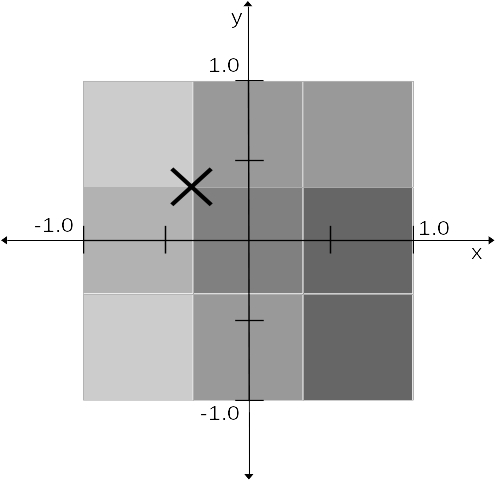
\includegraphics[width=0.5\linewidth]{images/schwerpunkt_ansatz.jpg}
    \caption{Illustration des Schwerpunktes im 3x3 Fotowiderstand-Array.}
    \label{fig:schwerpunkt}
\end{figure}
\begin{align}
    Q = \begin{pmatrix}
            q_{00} & q_{01} & q_{02} \\
            q_{10} & q_{11} & q_{12} \\
            q_{20} & q_{21} & q_{22}
    \end{pmatrix}
    \label{formular:pictureAsFormular}
\end{align}
Der Schwerpunkt $(X_Q, Y_Q)$ in einem Bild $Q$ (Formel \ref{formular:pictureAsFormular}) ist über die Helligkeit in den einzelnen Pixel definiert. Der Pixel $q_{11}$ bildet den Nullpunkt des Koordinatensystems.
Dann ist relativ zur Gesamthelligkeit $P = \sum_{i,j} q_{i,j}$, $X_Q=\frac{\sum_{i=0}^{2} q_{i,2} - \sum_{i=0}^{2} q_{i,0}}{P}$ die horizontale Komponente
und $Y_Q = \frac{\sum_{i=0}^{2} q_{0,i} - \sum_{i=0}^{2} q_{2,i}}{P}$ die vertikale Komponente des Schwerpunktes \cite{schwerpunktAnsatz}.
\newline
\newline
Ähnlich zur Helligkeitsverteilung wird das Feature mit einer Zeithistorie erweitert durch die multiple Anwendung auf verschiedene Zeitfenster, wobei die Anzahl der Zeitfenster variiert werden kann. Die
einzelnen Schwerpunkte innerhalb eines Zeitfensters werden über den Durchschnitt zusammengefasst.
\newline
\newline
Sollte die Anzahl der Bilder einer Handgeste ein Vielfaches von der Anzahl der Zeitfenster sein, wird die gleiche Anzahl an Bilder auf jedes Zeitfenster verteilt. Ansonsten werden Überschüsse einem Muster
nach bestimmten Zeitfenstern zugeordnet. Bei 5 Zeitfenstern wird der erste Überschuss dem letzten Zeitfenster zugeordnet, der zweite dem ersten, der dritte dem dritten, der vierte dem zweiten.
\newline
\newline
Die Schwerpunktverteilung ist durch die Dividierung mit $P$ invariant gegenüber Skalierung der Helligkeit, jedoch nicht gegenüber einen Offset. Alternativ kann $P$ weggelassen werden, damit ausschließlich
mit Integer gearbeitet wird. Dadurch können größere Bäume generiert werden (Kapitel \ref{sec:eval_size}) und die Feature-Extrahierung ist schneller (Kapitel \ref{sec:eval_speed}). Die Schwerpunktverteilung
mit Integer ist durch das weglassen von $P$ invariant gegenüber einen Offset $O$, da $\sum_{i=0}^{2}(q_{i,2} + O) - \sum_{i=0}^{2}(q_{i,0} + O)\ =\ \sum_{i=0}^{2} q_{i,2} - \sum_{i=0}^{2} q_{i,0} = X_Q$ ist und analog
für $Y_Q$. Der Ansatz mit den Ganzzahlen produziert Schwerpunkte in $[-3072, 3072]^2$ und der Ansatz mit Gleitkommazahlen produziert Schwerpunkte in $[-1, 1]^2$.
